\chapter{Implementierung}

	In diesem Kapitel werden einige Implementationsdetails dargestellt und erläutert, welche entweder einen kritischen Aspekt des Projekts darstellen oder von hoher Relevanz für den Erfolg des Projektes sind. 
	
	\section{Controller Interfaces}
	
		Wie bereits erwähnt sind die sog. Controller in einer \acs{MVC} Architektur für den Behandlung von Benutzereingaben zuständig. Im Falle einer \acs{REST}ful \acs{API} -- hier durch Spring umgesetzt -- dienen Controller dem Zweck, alle eingehenden \acs{HTTP} Anfragen zu behandeln. Dafür bietet Spring Annotationen, mit dessen Hilfe eindeutig definiert werden kann, wie die Anfrage auszusehen hat. Diese Definition eines sog. Endpoints beinhaltet immer einen Pfad, unter welchem der Endpoint erreicht werden kann, und eine \acs{HTTP} Methode. Es kann zusätzlich noch festgelegt werden, welche \acs{HTTP} Header bei einer Anfrage angegeben werden sollen und welcher \acs{MIME} Type zurück gegeben wird.
		
		\autoref{code:CityApi} zeigt beispielhaft, wie eine solche Definition eines Endpoints aussehen kann. Die eigentliche Beschreibung des Endpoints wird durch die Annotation \lstinline|@GetMapping| beschrieben. 	
		
		Um jedoch eine ausführlichere Beschreibung des Endpoints zu erstellen, können die von Swagger bereitgestellten Annotation verwendet werden. So lassen sich beispielsweise die Parameter, die Rückgabewerte aber auch die Authentifizierungsmethode beschreiben. Außerdem lassen sich noch Beschreibungen einfügen, um die Benutzung der \acs{API} zu erleichtern und zu dokumentieren. Für die City \acs{API} wird ein String als Parameter benötigt, mit dessen Hilfe die entsprechende Stadt zurückgegebene werden kann. Außerdem wird ein \acs{API} Key benötigt, um sich zu authentifizieren. 
		
		\lstinputlisting[
			label=code:CityApi,
			caption=Nutzung der beschriebenen Annotationen eines Controllers am Beispiel der City API,
			captionpos=b,               % Position, an der die Caption angezeigt wird t(op) oder b(ottom)
			style=EigenerJavaStyle,     % Eigener Style der vor dem Dokument festgelegt wurde
		]{code/CityApi.java}
		
	\section{Authentifizierung}
	
		\begin{figure}[ht!]
			\centering
			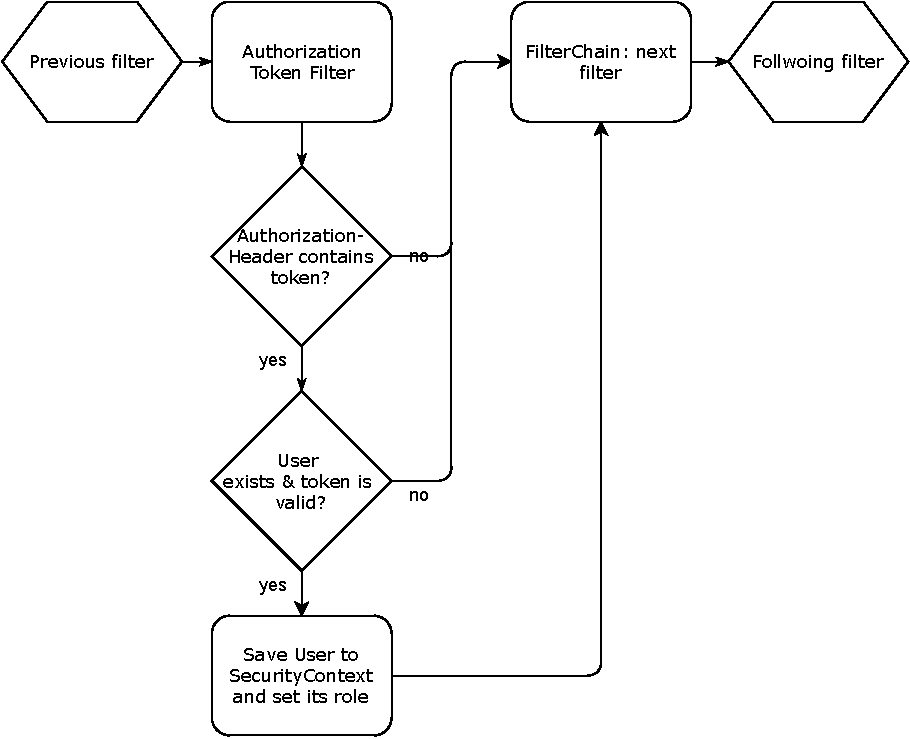
\includegraphics[width=1\textwidth]{images/authorization-flow-chart.pdf}
			\caption{Authentifizierungsprozess von \textit{Travlyn} mittels Spring Security Filter Chain}
			\label{fig:authenticationProcess}
		\end{figure} 
		
		\textit{Travlyn} stellt insgesamt zwei verschiedene Authentifizierungsrollen bereit. Wie \autoref{fig:UCD} zeigt, gibt es zum einen die Rolle des \acs{API}-Benutzers und die des registrierten Benutzers. Dem API Benutzer ist es erlaubt, Informationen wie beispielsweise über Trips anzufragen, wohingegen ein registrierter Benutzer auch die Möglichkeit hat, einen Trip zu erstellen. 
		
		Der Prozess der Authentifizierung basiert bei \textit{Travlyn} auf sog. Tokens. Sobald sich ein Benutzer registriert oder anmeldet, wird ein Token generiert -- das Token besteht aus 32 Zeichen und Ziffern und besitzt zudem ein Ablaufdatum, welches bei Überschreiten das Token als ungültig gekennzeichnet --, auf der Datenbank abgespeichert und zurück an den Benutzer gesendet. Um nun Endpoints anzufragen, welche eine Authentifizierung benötigen, wird dieses Token im \lstinline|Authorization|-Header im Format \lstinline|Bearer <token string>| gesendet. Auf dem Server erfolgt nun die Validierung des Tokens. So kann außerdem festgestellt werden, wer eine bestimmte Aktion ausgeführt hat. 
		
		Spring stellt für diesen Prozess einen Mechanismus bereit, um diese Authentifizierung möglichst einfach umzusetzen: Bevor eine Anfrage an einen bestimmten Endpoint zugelassen und die entsprechende Controller-Methode (wie bei \autoref{code:CityApi} beispielhaft gezeigt) aufgerufen wird, durchläuft diese Anfrage eine Reihe von Filtern. Diese sog. Filter Chain beinhaltet unter Anderem auch Authentifizierungsmechanismen, die sich eigens definieren lassen. So wurde für \textit{Travlyn} ein Filter namens \lstinline|AuthenticationTokenFilter| entwickelt, der dazu dient, das Token aus dem \acs{HTTP}-Header zu extrahieren und zu validieren. 
		
		Wenn das Token valide ist und auch der korrekten Benutzerrolle -- \acs{API}- oder registrierter Nutzer -- zugeordnet werden kann, wird die Anfrage an die entsprechende Controller Methode weitergeleitet und der entsprechende Nutzer im sog. \lstinline|SecurityContext| gespeichert, sodass auf die Rolle des Benutzers und auch auf den Benutzer selbst beim Prozessieren der Anfrage zugegriffen werden kann. Ist dies nicht der Fall, so wird diese Anfrage als nicht-authentifiziert markiert. \autoref{fig:authenticationProcess} visualisiert den Authentifizierungsprozess, wie er bei \textit{Travlyn} umgesetzt wurde.
		
		Um die zugelassenen Benutzerrollen für einen Endpoint der \acs{API} festzulegen, stellt das Modul Spring Security unter anderem die Annotation \lstinline|@PreAuthorize| zur Verfügung. Als Parameter wird ein in der \ac{SpEL} geschriebener Ausdruck übergeben, wie beispielsweise \lstinline|hasRole(API_USER)| in \autoref{code:CityApi}. So lässt sich die gesendete Authentisierung des Benutzers automatisiert überprüfen. 
		
